\documentclass[
  article,
  a4paper,
  12pt,
  oneside,
  fleqn
]{abntex2}

\usepackage[ABNTNum=brkt]{unoesc-article}

\addbibresource{referencias.bib}

\titulo{SISTEMA DE GESTÃO E RASTREABILIDADE DE CARTÕES DE AUXÍLIO}

\autor{
  Alexandre Reitemeyer\thanks{\affil{Curso de Sistemas de Informação, UNOESC, Chapecó}\sep\email{alexandre.reitemeyer@unoesc.edu.br}} \\
  Beatriz Miranda\thanks{\affil{Curso de Sistemas de Informação, UNOESC, Chapecó}\sep\email{beatriz.miranda@unoesc.edu.br}} \\
  Jessé Chaves\thanks{\affil{Curso de Sistemas de Informação, UNOESC, Chapecó}\sep\email{jesse.chaves@unoesc.edu.br}} \\
  Lucas Santos Magro\thanks{\affil{Curso de Sistemas de Informação, UNOESC, Chapecó}\sep\email{lucas.magro@unoesc.edu.br}}
}

\data{Chapecó, abril de 2026}

\begin{document}



\pretextual

\begin{paginadetitulo}
    \begin{ambienteresumo}
        Este documento apresenta a documentação completa do projeto AuxílioPay, um sistema web para gestão e rastreabilidade de cartões de auxílio desenvolvido na disciplina de Práticas em Sistemas de Informação. O trabalho contempla a descrição do sistema proposto, o levantamento de requisitos funcionais e não funcionais, o modelo entidade-relacionamento, os diagramas de classes e de caso de uso, a descrição das telas do protótipo navegável e o cronograma de desenvolvimento. O sistema visa resolver os desafios de controle, segurança e rastreabilidade enfrentados por organizações que distribuem cartões físicos de auxílio, garantindo conformidade com a LGPD.
        \palavraschave{Cartões de Auxílio. Rastreabilidade. LGPD. Gestão de Benefícios. Protótipo.}
    \end{ambienteresumo}
\end{paginadetitulo}

\textual
\newpage

% =============================================================================
% SEÇÃO 1 — INTRODUÇÃO
% =============================================================================
\section{Introdução}

Organizações públicas e privadas que distribuem cartões físicos de auxílio --- alimentação, transporte, saúde --- enfrentam desafios críticos na gestão desses ativos. A ausência de visibilidade em tempo real sobre o status de cada cartão compromete a eficiência operacional e abre brechas para fraudes. Sem trilhas de auditoria adequadas, torna-se impossível rastrear quem detém a posse de um cartão em determinado momento, o que gera riscos de duplicidade de entregas e perda de controle patrimonial.

Além dos desafios operacionais, a conformidade com a Lei Geral de Proteção de Dados Pessoais (LGPD --- Lei nº 13.709/2018) impõe exigências rigorosas quanto ao tratamento de dados pessoais dos beneficiários. Informações sensíveis como CPF, endereço e dados de contato precisam ser armazenadas com criptografia adequada, e todas as operações sobre esses dados devem ser registradas e auditáveis.

Nesse contexto, este trabalho propõe o desenvolvimento do \textbf{AuxílioPay}: um sistema web centralizado para gestão e rastreabilidade do ciclo de vida completo de cartões de auxílio. A plataforma oferece controle de entregas e devoluções com responsabilidade única por cartão, geração automática de comprovantes em PDF, notificações inteligentes por e-mail e SMS, criptografia AES-256 para dados pessoais e conformidade integral com a LGPD, incluindo retenção de logs de auditoria por no mínimo dois anos.

% =============================================================================
% SEÇÃO 2 — DESCRIÇÃO DO SISTEMA
% =============================================================================
\section{Descrição do Sistema}

O AuxílioPay é uma plataforma web centralizada projetada para gerenciar o ciclo de vida completo de cartões de auxílio distribuídos por organizações. O sistema contempla os seguintes aspectos fundamentais:

\begin{itemize}
    \item \textbf{Responsabilidade única:} cada cartão é associado a exatamente um beneficiário responsável por vez. A transferência de responsabilidade só ocorre mediante registro formal no sistema;
    \item \textbf{Rastreabilidade completa:} todas as movimentações --- entrega, devolução e consultas --- são registradas com timestamp, identificação do administrador responsável e condição do cartão;
    \item \textbf{Geração automática de comprovantes:} o sistema gera comprovantes em formato PDF em menos de 5 segundos após cada operação de entrega ou devolução;
    \item \textbf{Consulta de status em tempo real:} qualquer administrador autorizado pode consultar o status atual de um cartão, incluindo seu histórico completo de movimentações;
    \item \textbf{Notificações automáticas:} o sistema envia notificações por e-mail e SMS aos beneficiários quando se aproximam os prazos de devolução de cartões;
    \item \textbf{Criptografia AES-256:} todos os dados pessoais dos beneficiários (CPF, telefone, endereço) são armazenados com criptografia AES-256;
    \item \textbf{Autenticação de dois fatores (2FA):} administradores utilizam autenticação de dois fatores para acesso ao sistema, reduzindo riscos de acesso não autorizado;
    \item \textbf{Log de auditoria:} todas as operações são registradas em log de auditoria com retenção mínima de 2 anos, em conformidade com a LGPD.
\end{itemize}

% =============================================================================
% SEÇÃO 3 — REQUISITOS FUNCIONAIS E NÃO FUNCIONAIS
% =============================================================================
\section{Requisitos Funcionais e Não Funcionais}

Os requisitos a seguir foram levantados com base nas necessidades identificadas para o gerenciamento seguro e eficiente de cartões de auxílio, seguindo as boas práticas de engenharia de requisitos.

\subsection{Requisitos Funcionais}

\begin{itemize}
    \item \textbf{RF-01: Registrar Entrega de Cartão}
    \begin{itemize}
        \item O sistema deve permitir que o Administrador registre a entrega de um cartão de auxílio para um Beneficiário;
        \item O sistema deve registrar a data, hora e identificação do Beneficiário que recebeu o cartão;
        \item O sistema deve armazenar o número de série/identificação do cartão entregue.
    \end{itemize}

    \item \textbf{RF-02: Registrar Devolução de Cartão}
    \begin{itemize}
        \item O sistema deve permitir que o Administrador registre a devolução de um cartão de auxílio;
        \item O sistema deve registrar a data, hora e condição do cartão devolvido;
        \item O sistema deve validar se o cartão foi previamente entregue antes de permitir seu registro de devolução.
    \end{itemize}

    \item \textbf{RF-03: Consultar Status do Cartão}
    \begin{itemize}
        \item O sistema deve permitir que o Administrador consulte o status de qualquer cartão em tempo real;
        \item O sistema deve exibir informações sobre a data de entrega, beneficiário responsável e histórico completo;
        \item O Administrador deve ter acesso ao histórico completo de movimentação de cartões.
    \end{itemize}

    \item \textbf{RF-04: Criar Notificação de Devolução}
    \begin{itemize}
        \item O sistema deve permitir ao Administrador criar e configurar notificações de devolução para beneficiários;
        \item O sistema deve permitir configurar o prazo de devolução e os canais de comunicação (e-mail, SMS, etc.);
        \item O sistema deve registrar as notificações criadas, enviadas e confirmadas com data e conteúdo.
    \end{itemize}

    \item \textbf{RF-05: Controlar Responsabilidade do Cartão}
    \begin{itemize}
        \item O sistema deve manter registro de quem está com o cartão em cada momento;
        \item O sistema deve impedir que múltiplos beneficiários sejam responsáveis pelo mesmo cartão simultaneamente;
        \item O sistema deve permitir transferência de responsabilidade com registro de auditoria.
    \end{itemize}
\end{itemize}

\subsection{Requisitos Não Funcionais}

\begin{itemize}
    \item \textbf{RNF-01: Disponibilidade}
    \begin{itemize}
        \item O sistema deve estar disponível 24/7 com tempo de parada máximo de 2 horas por mês para manutenção;
        \item O sistema deve ter backup automático a cada 24 horas;
        \item O sistema deve ter plano de recuperação de desastres (\textit{disaster recovery}).
    \end{itemize}

    \item \textbf{RNF-02: Segurança}
    \begin{itemize}
        \item Todos os dados pessoais do Beneficiário devem ser protegidos com criptografia AES-256;
        \item O sistema deve implementar autenticação de dois fatores para o Administrador;
        \item Deve haver registro de auditoria de todas as operações com timestamp e identificação do usuário;
        \item O sistema deve cumprir com a LGPD (Lei Geral de Proteção de Dados).
    \end{itemize}

    \item \textbf{RNF-03: Performance}
    \begin{itemize}
        \item O tempo de resposta para consultar o status de um cartão não deve exceder 2 segundos;
        \item O sistema deve suportar processamento de até 1.000 requisições simultâneas;
        \item A geração de comprovantes não deve exceder 5 segundos.
    \end{itemize}

    \item \textbf{RNF-04: Confiabilidade}
    \begin{itemize}
        \item Taxa de erro máxima de 0,1\% em registros de transações;
        \item Validação automática de integridade de dados;
        \item Sistema de alertas para detecção de anomalias.
    \end{itemize}

    \item \textbf{RNF-05: Rastreabilidade}
    \begin{itemize}
        \item Todos os movimentos de cartão devem estar vinculados a um timestamp preciso;
        \item Deve ser possível gerar relatórios de auditoria a qualquer momento;
        \item Retenção de logs por no mínimo 2 anos.
    \end{itemize}
\end{itemize}

% =============================================================================
% SEÇÃO 4 — MODELO ENTIDADE-RELACIONAMENTO
% =============================================================================
\section{Modelo Entidade-Relacionamento}

O modelo entidade-relacionamento (MER) do sistema foi projetado para garantir a rastreabilidade completa de todas as operações e a integridade referencial dos dados. O modelo é composto por sete entidades principais que se relacionam em torno da entidade central \textbf{MOVIMENTACAO}, responsável por registrar cada operação de entrega ou devolução de cartão.

A \cref{fig:mer} apresenta o diagrama completo do modelo entidade-relacionamento do sistema.

\begin{figure}[htb]
    \caption{\label{fig:mer}Modelo Entidade-Relacionamento do sistema AuxílioPay}
    \begin{center}
        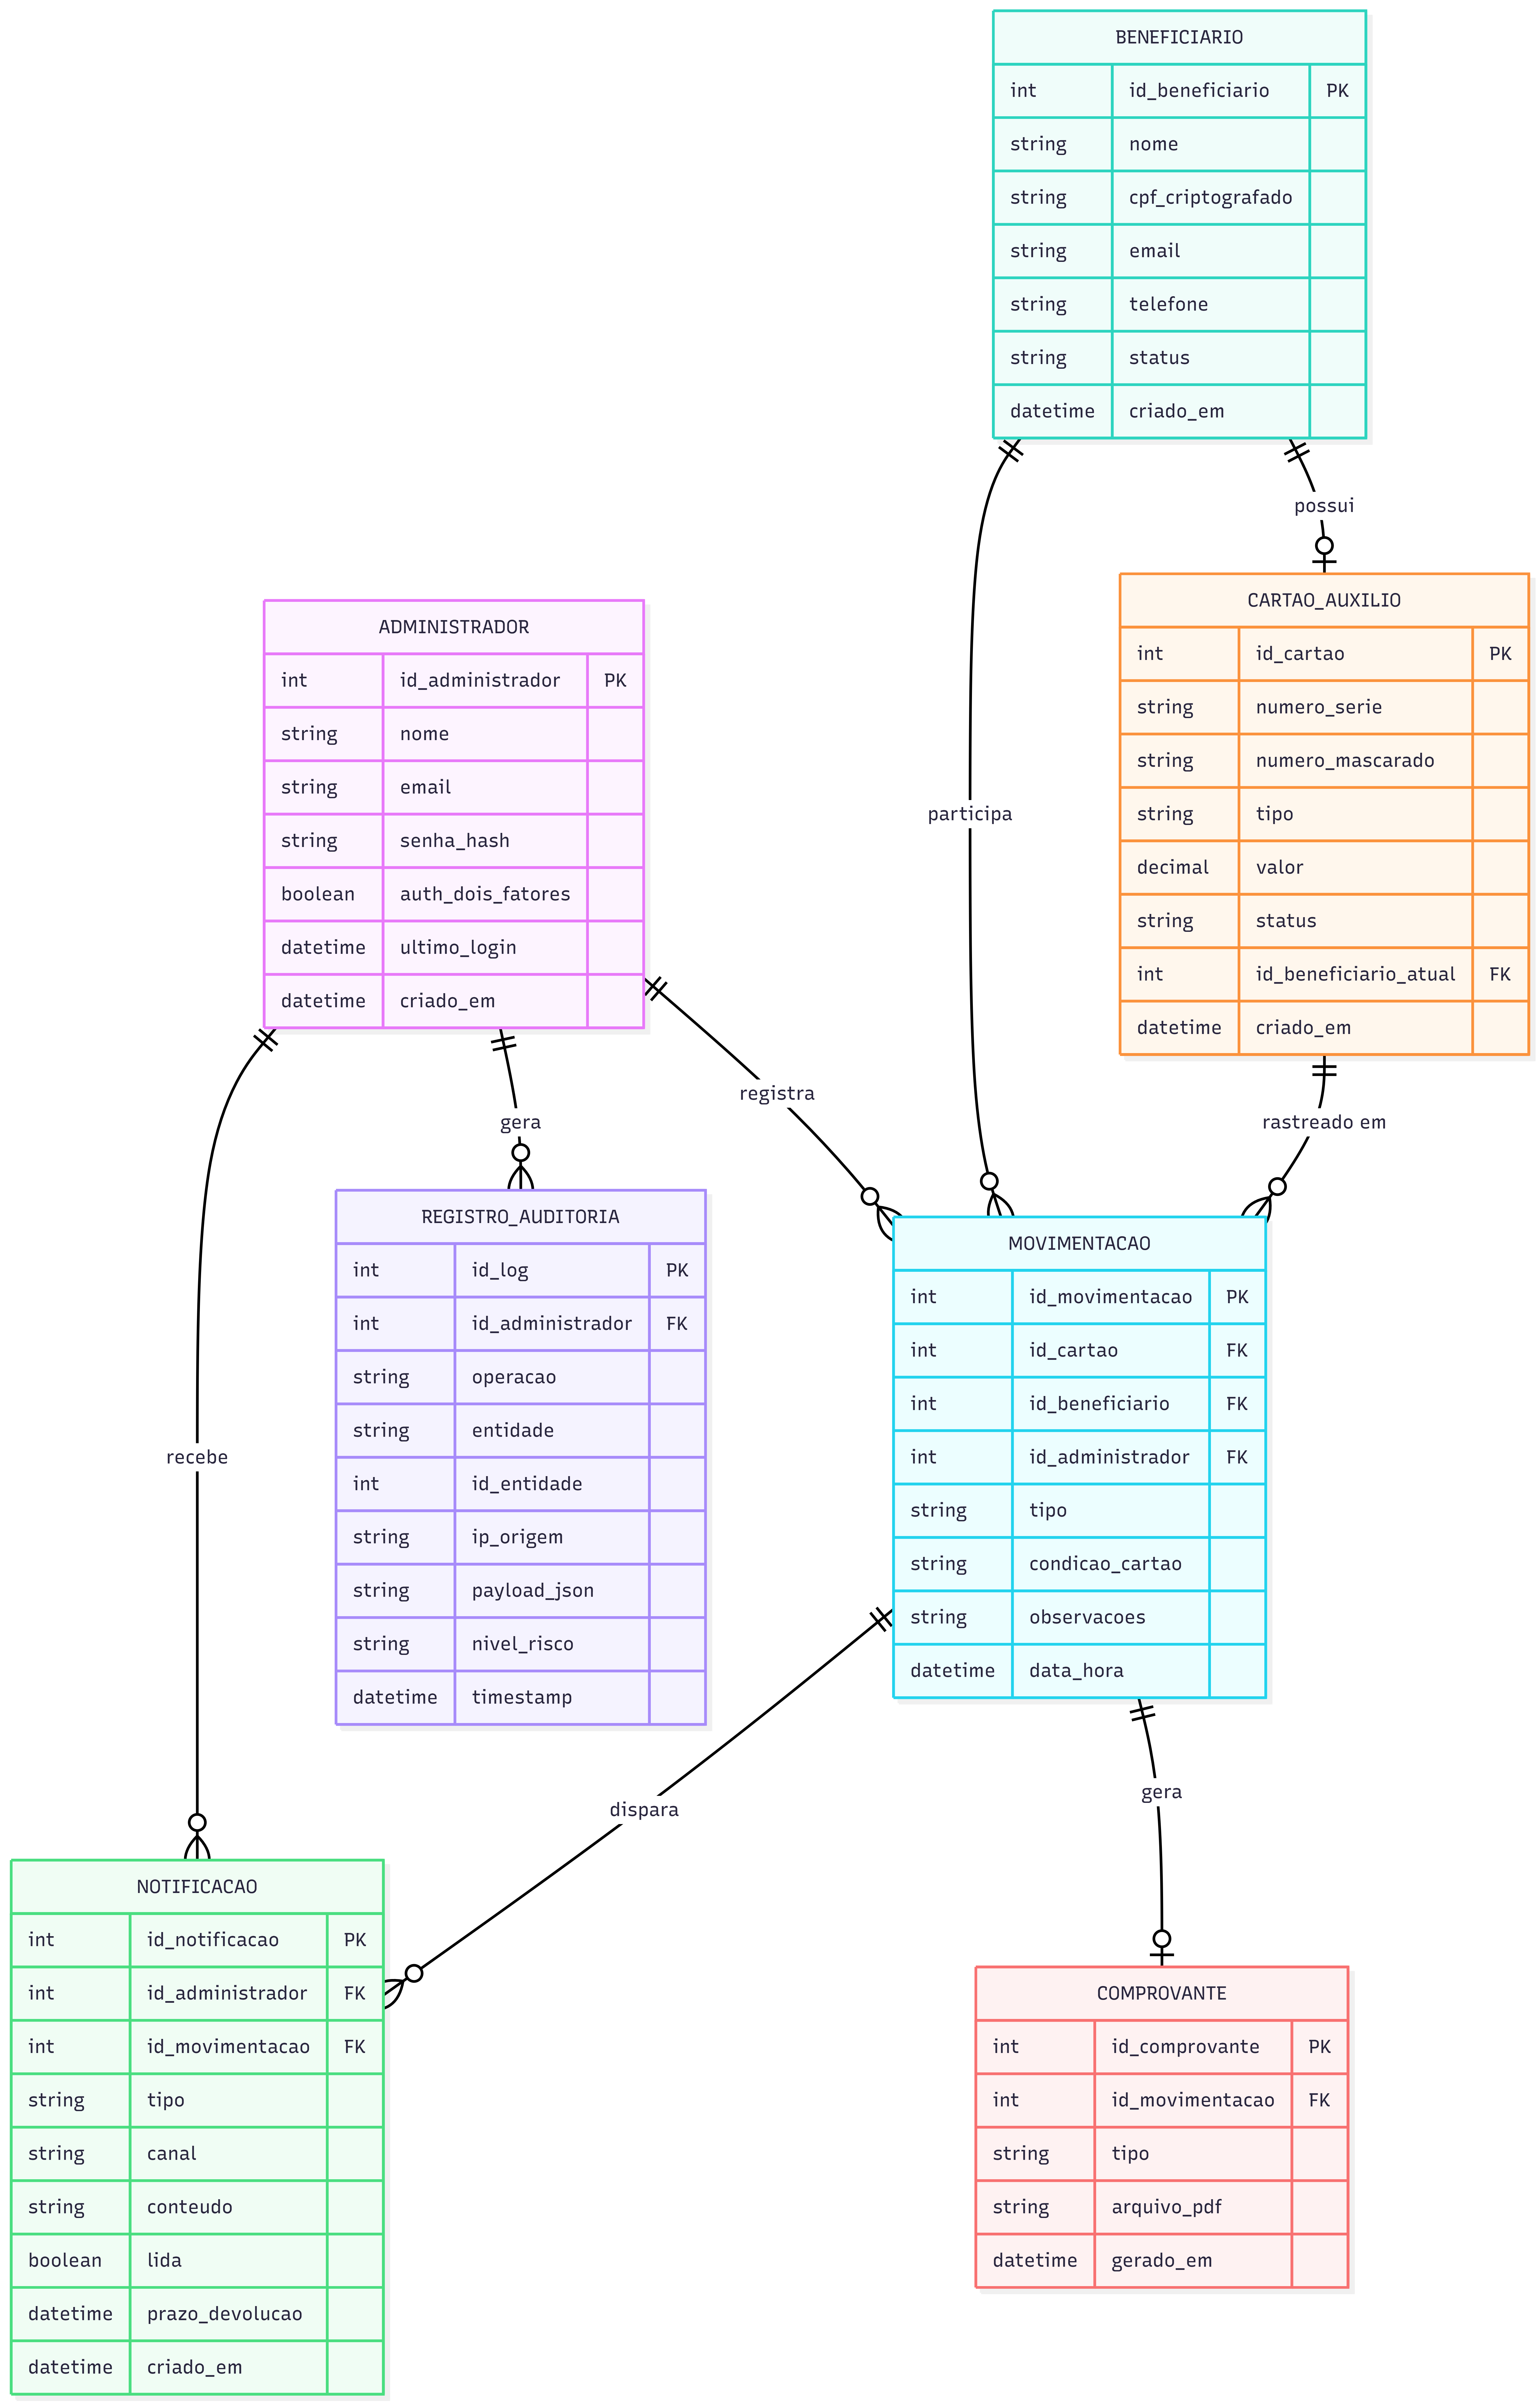
\includegraphics[width=16cm]{imagens/ModeloER.png}
    \end{center}
    \fonte{Acervo Pessoal (2026).}
\end{figure}

A seguir são descritas as entidades que compõem o modelo:

\begin{itemize}
    \item \textbf{ADMINISTRADOR:} representa o usuário que opera o sistema. É responsável por registrar entregas e devoluções, receber notificações e gerar registros de auditoria;

    \item \textbf{BENEFICIARIO:} representa a pessoa física que recebe o cartão de auxílio. Pode possuir no máximo um cartão ativo por vez;

    \item \textbf{CARTAO\_AUXILIO:} armazena os dados de cada cartão, como número de série, tipo de benefício, valor e status atual. Está vinculado ao beneficiário responsável no momento;

    \item \textbf{MOVIMENTACAO:} entidade central do modelo. Registra cada operação de entrega ou devolução, vinculando o administrador, o beneficiário e o cartão envolvidos, além da data/hora e condição do cartão;

    \item \textbf{NOTIFICACAO:} registra os alertas enviados sobre prazos de devolução, incluindo o canal de envio (e-mail ou SMS) e se a notificação foi lida;

    \item \textbf{REGISTRO\_AUDITORIA:} armazena o log de todas as operações do sistema, com dados como IP de origem, operação executada e nível de risco, garantindo conformidade com a LGPD;

    \item \textbf{COMPROVANTE:} representa o comprovante em PDF gerado automaticamente após cada operação de entrega ou devolução.
\end{itemize}

A \cref{tab:entidades} resume os atributos de cada entidade.

\begin{table}[htb]
\caption{\label{tab:entidades}Entidades do sistema e seus atributos principais}
\centering
\footnotesize
\begin{tabular}{p{4cm}p{10cm}}
\toprule
\textbf{Entidade} & \textbf{Atributos} \\
\midrule
ADMINISTRADOR & id, nome, email, senha\_hash, auth\_dois\_fatores, ultimo\_login, criado\_em \\
\midrule
BENEFICIARIO & id, nome, cpf\_criptografado, email, telefone, status, criado\_em \\
\midrule
CARTAO\_AUXILIO & id, numero\_serie, numero\_mascarado, tipo, valor, status, id\_beneficiario\_atual (FK), criado\_em \\
\midrule
MOVIMENTACAO & id, id\_cartao (FK), id\_beneficiario (FK), id\_administrador (FK), tipo, condicao\_cartao, observacoes, data\_hora \\
\midrule
NOTIFICACAO & id, id\_administrador (FK), id\_movimentacao (FK), tipo, canal, conteudo, lida, prazo\_devolucao, criado\_em \\
\midrule
REGISTRO\_AUDITORIA & id, id\_administrador (FK), operacao, entidade, id\_entidade, ip\_origem, payload\_json, nivel\_risco, timestamp \\
\midrule
COMPROVANTE & id, id\_movimentacao (FK), tipo, arquivo\_pdf, gerado\_em \\
\bottomrule
\end{tabular}
\end{table}

\subsection{Relacionamentos}

Os relacionamentos entre as entidades do sistema são:

\begin{itemize}
    \item \textbf{ADMINISTRADOR} registra \textbf{MOVIMENTACAO} (1 para N);
    \item \textbf{ADMINISTRADOR} recebe \textbf{NOTIFICACAO} (1 para N);
    \item \textbf{ADMINISTRADOR} gera \textbf{REGISTRO\_AUDITORIA} (1 para N);
    \item \textbf{BENEFICIARIO} participa de \textbf{MOVIMENTACAO} (1 para N);
    \item \textbf{BENEFICIARIO} possui \textbf{CARTAO\_AUXILIO} (1 para 0..1);
    \item \textbf{CARTAO\_AUXILIO} é rastreado em \textbf{MOVIMENTACAO} (1 para N);
    \item \textbf{MOVIMENTACAO} dispara \textbf{NOTIFICACAO} (1 para N);
    \item \textbf{MOVIMENTACAO} gera \textbf{COMPROVANTE} (1 para 0..1).
\end{itemize}

% =============================================================================
% SEÇÃO 5 — DIAGRAMA DE CLASSES
% =============================================================================
\section{Diagrama de Classes}

O diagrama de classes representa a estrutura estática do sistema, definindo as classes, seus atributos, métodos e os relacionamentos entre elas.

\begin{figure}[htb]
    \caption{\label{fig:classes}Diagrama de Classes do sistema AuxílioPay}
    \begin{center}
        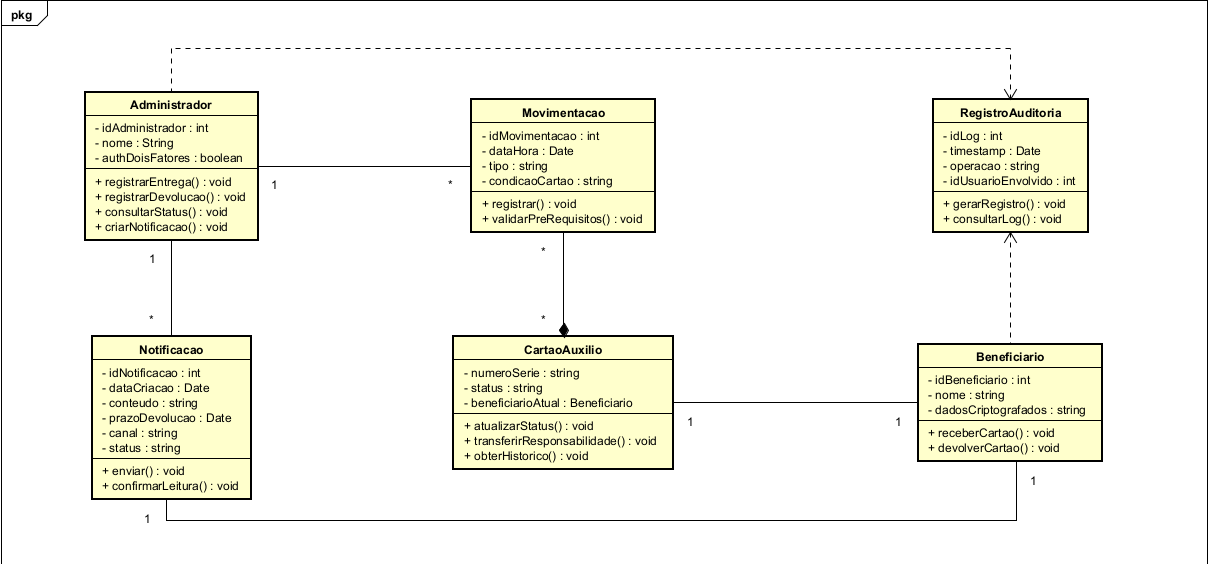
\includegraphics[width=15cm]{imagens/DiagramaDeClasses.png}
    \end{center}
    \fonte{Acervo Pessoal (2026).}
\end{figure}

As principais classes do sistema são descritas a seguir:

\begin{itemize}
    \item \textbf{Administrador:}
    \begin{itemize}
        \item Atributos: \texttt{id}, \texttt{nome}, \texttt{authDoisFatores};
        \item Métodos: \texttt{registrarEntrega()}, \texttt{registrarDevolucao()},\\ \texttt{consultarStatus()}, \texttt{criarNotificacao()}.
    \end{itemize}

    \item \textbf{Beneficiario:}
    \begin{itemize}
        \item Atributos: \texttt{id}, \texttt{nome}, \texttt{dadosCriptografados};
        \item Métodos: \texttt{receberCartao()}, \texttt{devolverCartao()}.
    \end{itemize}

    \item \textbf{CartaoAuxilio:}
    \begin{itemize}
        \item Atributos: \texttt{numeroSerie}, \texttt{status}, \texttt{beneficiarioAtual};
        \item Métodos: \texttt{atualizarStatus()}, \texttt{transferirResponsabilidade()},\\ \texttt{obterHistorico()}.
    \end{itemize}

    \item \textbf{Movimentacao:}
    \begin{itemize}
        \item Atributos: \texttt{id}, \texttt{dataHora}, \texttt{tipo}, \texttt{condicaoCartao};
        \item Métodos: \texttt{registrar()}, \texttt{validarPreRequisitos()}.
    \end{itemize}

    \item \textbf{Notificacao:}
    \begin{itemize}
        \item Atributos: \texttt{id}, \texttt{conteudo}, \texttt{canal}, \texttt{prazo};
        \item Métodos: \texttt{enviar()}, \texttt{confirmarLeitura()}.
    \end{itemize}

    \item \textbf{RegistroAuditoria:}
    \begin{itemize}
        \item Atributos: \texttt{id}, \texttt{timestamp}, \texttt{operacao};
        \item Métodos: \texttt{gerarRegistro()}, \texttt{consultarLog()}.
    \end{itemize}
\end{itemize}

% =============================================================================
% SEÇÃO 6 — DIAGRAMA DE CASO DE USO
% =============================================================================
\section{Diagrama de Caso de Uso}

O diagrama de caso de uso descreve as interações entre os atores do sistema e as funcionalidades disponíveis.

\begin{figure}[htb]
    \caption{\label{fig:caso_uso}Diagrama de Caso de Uso do sistema AuxílioPay}
    \begin{center}
        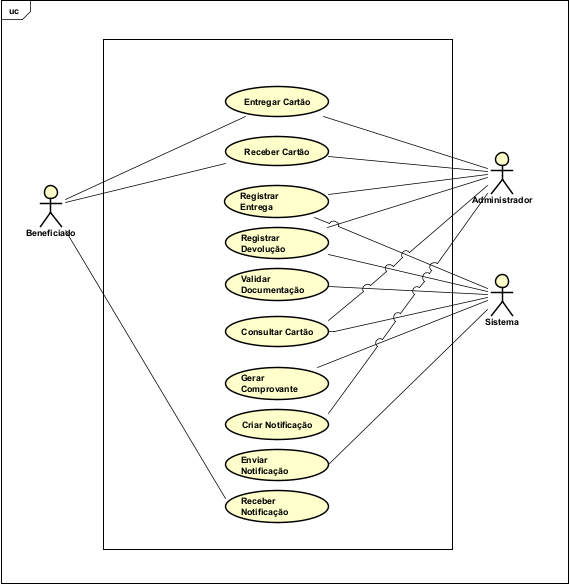
\includegraphics[width=15cm]{imagens/DiagramaCasoDeUso.png}
    \end{center}
    \fonte{Acervo Pessoal (2026).}
\end{figure}

\subsection{Atores}

O sistema possui três atores principais:

\begin{itemize}
    \item \textbf{Beneficiário:} pessoa física que recebe e devolve os cartões de auxílio;
    \item \textbf{Administrador:} responsável por operar o sistema, registrar entregas e devoluções, e gerenciar notificações;
    \item \textbf{Sistema:} componente automatizado responsável por validações, geração de comprovantes e envio de notificações.
\end{itemize}

\subsection{Casos de Uso}

Os casos de uso identificados e seus respectivos atores são:

\begin{itemize}
    \item \textbf{Entregar Cartão} e \textbf{Receber Cartão:} envolvem o Beneficiário e o Administrador;
    \item \textbf{Registrar Entrega}, \textbf{Registrar Devolução} e \textbf{Validar Documentação:} envolvem o Administrador e o Sistema;
    \item \textbf{Consultar Cartão} e \textbf{Gerar Comprovante:} envolvem o Administrador e o Sistema;
    \item \textbf{Criar Notificação}, \textbf{Enviar Notificação} e \textbf{Receber Notificação:} envolvem o Administrador, o Sistema e o Beneficiário.
\end{itemize}

% =============================================================================
% SEÇÃO 7 — DESCRIÇÃO DO PROTÓTIPO
% =============================================================================
\section{Descrição do Protótipo}

Um protótipo funcional foi desenvolvido para demonstrar o fluxo completo do sistema proposto por meio de telas interativas. A seguir são descritas as telas que compõem o protótipo e o que o usuário visualiza em cada uma delas.

\subsection{Telas do Protótipo}

\begin{itemize}
    \item \textbf{Dashboard:} tela inicial que exibe indicadores resumidos --- total de cartões cadastrados, cartões entregues, cartões disponíveis e cartões bloqueados. Apresenta também um gráfico de barras com as movimentações mensais, um gráfico de rosca com a distribuição por tipo de benefício, um feed com as atividades mais recentes do sistema e um relógio com a data e hora atuais;

    \item \textbf{Cartões:} tela com uma tabela que lista todos os cartões cadastrados, com campo de busca por texto, filtro por status (Cadastrado, Disponível, Entregue, Devolvido, Bloqueado), ordenação por qualquer coluna e paginação com 8 registros por página. Ao clicar em um cartão, abre-se um painel de detalhes que mostra uma visualização do cartão físico, um indicador visual de status (Cadastrado $\rightarrow$ Disponível $\rightarrow$ Entregue $\rightarrow$ Devolvido) e o histórico completo de movimentações daquele cartão;

    \item \textbf{Nova Entrega:} tela com um formulário em 3 etapas. Na primeira etapa, o administrador informa os dados do beneficiário e o sistema valida o CPF. Na segunda etapa, é selecionado o cartão disponível para entrega, com uma pré-visualização do cartão escolhido. Na terceira etapa, é exibido um resumo da operação com campo de assinatura digital para confirmação;

    \item \textbf{Devolução:} tela onde o administrador busca um cartão que esteja com status ``Entregue'', seleciona a condição de devolução do cartão e, ao confirmar, visualiza um comprovante de devolução gerado automaticamente;

    \item \textbf{Beneficiários:} tela que permite cadastrar, editar, consultar e excluir beneficiários. Possui campo de busca por nome e filtro por status. Ao selecionar um beneficiário, abre-se um painel lateral com o histórico completo de cartões recebidos e devolvidos por aquele beneficiário;

    \item \textbf{Relatórios:} tela com filtros por período de data, botão de exportação para arquivo CSV e um ranking dos beneficiários com maior volume de movimentações;

    \item \textbf{Notificações:} tela que centraliza todos os alertas do sistema, com opções de configuração por canal de envio (e-mail e SMS) por meio de botões de ativar/desativar;

    \item \textbf{Auditoria:} tela que exibe o log completo de operações do sistema em formato de tabela, com filtros por tipo de operação, data e nível de risco. Cada linha pode ser expandida para exibir os detalhes completos da operação registrada e seu respectivo indicador de risco;

    \item \textbf{Configurações:} tela de configurações do perfil do administrador, com opção de ativar ou desativar a autenticação de dois fatores (exibindo um QR code para configuração), preferências de notificação e informações gerais do sistema.
\end{itemize}

\subsection{Recursos Gerais da Interface}

Além das telas descritas, o protótipo apresenta os seguintes recursos presentes em toda a interface:

\begin{itemize}
    \item Barra de busca global acessível por atalho de teclado;
    \item Mensagens de confirmação e alerta após cada operação realizada;
    \item Tutorial guiado para novos usuários na primeira utilização;
    \item Indicadores visuais de carregamento enquanto os dados são apresentados;
    \item Mensagens ilustrativas quando não há dados a serem exibidos em uma tela;
    \item Layout adaptado para uso em dispositivos móveis, com menu de navegação inferior.
\end{itemize}

% =============================================================================
% SEÇÃO 8 — CRONOGRAMA DE DESENVOLVIMENTO
% =============================================================================
\section{Cronograma de Desenvolvimento}

O cronograma de desenvolvimento foi planejado em 8 semanas, distribuindo as tarefas entre quatro desenvolvedores, conforme apresentado na \cref{tab:cronograma}.

\begin{table}[htb]
\caption{\label{tab:cronograma}Cronograma de desenvolvimento do sistema}
\centering
\footnotesize
\begin{tabular}{c c p{7.5cm} c}
\toprule
\textbf{Semana} & \textbf{Responsável} & \textbf{Tarefa} & \textbf{Requisito} \\
\midrule
1--2 & Dev 1 & Configurar repositório, CI/CD, ambiente Cloud e banco de dados PostgreSQL & Estrutura \\
1--2 & Dev 2 & Criar serviço de autenticação com 2FA e criptografia AES-256 & RNF-02 \\
1--2 & Dev 3 & Configurar projeto front-end React, roteamento e tela de login & Estrutura / RNF-02 \\
1--2 & Dev 4 & Criar painel base (Sidebar, Header) e configurar framework de testes & Estrutura \\
\midrule
3--4 & Dev 1 & Desenvolver API de Efetuar Entrega com validação de responsabilidade única & RF-01, RF-05 \\
3--4 & Dev 2 & Desenvolver API de Consultar Status e registro de auditoria global & RF-03, RNF-05 \\
3--4 & Dev 3 & Criar tela de Nova Entrega com formulários de busca e vinculação de cartão & RF-01 \\
3--4 & Dev 4 & Criar tela de Consultar Status integrada com API (carregamento < 2s) & RF-03, RNF-03 \\
\midrule
5--6 & Dev 1 & Desenvolver API de Registrar Devolução com validação de status & RF-02 \\
5--6 & Dev 2 & Desenvolver geração de comprovante PDF (< 5 segundos) & RNF-03 \\
5--6 & Dev 3 & Criar tela de Devolução e visualização de histórico completo & RF-02, RF-03 \\
5--6 & Dev 4 & Criar relatórios de auditoria e testes de estresse & RNF-05 \\
\midrule
7--8 & Dev 1 & Otimizar queries, configurar backup 24h e alertas de anomalia & RNF-01, RNF-04 \\
7--8 & Dev 2 & Desenvolver módulo de notificações com e-mail/SMS (AWS SES, Twilio) & RF-04 \\
7--8 & Dev 3 & Criar tela de Gestão de Notificações e polir interface UX & RF-04 \\
7--8 & Dev 4 & Executar testes de carga (1.000 requisições simultâneas) e corrigir gargalos & RNF-03 \\
\bottomrule
\end{tabular}
\end{table}

% =============================================================================
% SEÇÃO 9 — CONSIDERAÇÕES FINAIS
% =============================================================================
\section{Considerações Finais}

O presente trabalho apresentou o desenvolvimento do AuxílioPay, um sistema web para gestão e rastreabilidade de cartões de auxílio que endereça os desafios identificados na distribuição e controle desses ativos por organizações.

O sistema proposto contempla todas as necessidades levantadas durante a análise de requisitos: controle de responsabilidade única por cartão, rastreabilidade completa de movimentações, geração automática de comprovantes, notificações inteligentes para prazos de devolução e um robusto sistema de auditoria. A conformidade com a LGPD é garantida por meio da criptografia AES-256 para dados pessoais, autenticação de dois fatores para administradores e retenção de logs de auditoria por no mínimo dois anos, seguindo as melhores práticas de segurança recomendadas pela OWASP.

O protótipo funcional demonstra a viabilidade da proposta e apresenta o fluxo completo de trabalho --- desde o registro de entregas até a geração de relatórios de auditoria --- em uma interface moderna, responsiva e acessível.

Como trabalhos futuros, destacam-se: (i) a implementação completa do backend e integração com banco de dados; (ii) a integração com provedores de e-mail e SMS para o módulo de notificações; e (iii) a implantação em ambiente de produção com monitoramento e escalabilidade.



\end{document}
